% ============================================================
% Question Bank: ch06-01 Understanding and Using Scale Drawings
% Topic Title: Understanding and Using Scale Drawings
% CCSS: 7.G.A.1
% Questions: 30 (18 MC + 7 SA + 5 Graphical)
% ============================================================

% --- Multiple Choice Questions (18) ---

\begin{practiceQuestion}{6-1-q01}{mc}
\begin{questionText}
A map uses the scale $1$ cm $= 25$ km. Two towns are $6$ cm apart on the map. What is the actual distance?
\end{questionText}
\choiceA{$31$ km}
\choiceB{$125$ km}
\choiceC{$150$ km}
\choiceD{$175$ km}
\correctAnswer{C}
\explanation{Multiply the map distance by the scale factor: $6 \times 25 = 150$ km.}
\end{practiceQuestion}

\begin{practiceQuestion}{6-1-q02}{mc}
\begin{questionText}
A blueprint uses the scale $1$ in $= 6$ ft. A hallway is $3.5$ in long on the blueprint. What is the actual length?
\end{questionText}
\choiceA{$18$ ft}
\choiceB{$21$ ft}
\choiceC{$24$ ft}
\choiceD{$9.5$ ft}
\correctAnswer{B}
\explanation{$3.5 \times 6 = 21$ ft.}
\end{practiceQuestion}

\begin{practiceQuestion}{6-1-q03}{mc}
\begin{questionText}
A model airplane has a scale of $1:72$. The model's wingspan is $8$ inches. What is the actual wingspan?
\end{questionText}
\choiceA{$9$ inches}
\choiceB{$80$ inches}
\choiceC{$576$ inches}
\choiceD{$648$ inches}
\correctAnswer{C}
\explanation{Multiply by the scale factor: $8 \times 72 = 576$ inches.}
\end{practiceQuestion}

\begin{practiceQuestion}{6-1-q04}{mc}
\begin{questionText}
On a map, $2$ cm represents $50$ km. What is the scale factor?
\end{questionText}
\choiceA{$2$ km per cm}
\choiceB{$25$ km per cm}
\choiceC{$50$ km per cm}
\choiceD{$100$ km per cm}
\correctAnswer{B}
\explanation{Find the unit rate: $50 \div 2 = 25$ km per cm.}
\end{practiceQuestion}

\begin{practiceQuestion}{6-1-q05}{mc}
\begin{questionText}
A scale drawing uses $1$ cm $= 4$ m. A room is $5$ cm by $3$ cm on the drawing. What is the actual area of the room?
\end{questionText}
\choiceA{$15$ m$^2$}
\choiceB{$60$ m$^2$}
\choiceC{$192$ m$^2$}
\choiceD{$240$ m$^2$}
\correctAnswer{D}
\explanation{Actual dimensions: $5 \times 4 = 20$ m and $3 \times 4 = 12$ m. Area: $20 \times 12 = 240$ m$^2$.}
\end{practiceQuestion}

\begin{practiceQuestion}{6-1-q06}{mc}
\begin{questionText}
If a scale factor is $3$, how does the area of the actual figure compare to the area of the drawing?
\end{questionText}
\choiceA{$3$ times as large}
\choiceB{$6$ times as large}
\choiceC{$9$ times as large}
\choiceD{$12$ times as large}
\correctAnswer{C}
\explanation{When lengths scale by $k$, areas scale by $k^2$. So $3^2 = 9$ times as large.}
\end{practiceQuestion}

\begin{practiceQuestion}{6-1-q07}{mc}
\begin{questionText}
A park is $120$ m long. On a scale drawing, it is $8$ cm long. What scale does the drawing use?
\end{questionText}
\choiceA{$1$ cm $= 10$ m}
\choiceB{$1$ cm $= 12$ m}
\choiceC{$1$ cm $= 15$ m}
\choiceD{$1$ cm $= 20$ m}
\correctAnswer{C}
\explanation{$120 \div 8 = 15$. The scale is $1$ cm $= 15$ m.}
\end{practiceQuestion}

\begin{practiceQuestion}{6-1-q08}{mc}
\begin{questionText}
A scale drawing of a building uses $1$ in $= 10$ ft. The building is $85$ ft tall. How tall is it on the drawing?
\end{questionText}
\choiceA{$8$ in}
\choiceB{$8.5$ in}
\choiceC{$85$ in}
\choiceD{$850$ in}
\correctAnswer{B}
\explanation{Divide actual length by the scale factor: $85 \div 10 = 8.5$ in.}
\end{practiceQuestion}

\begin{practiceQuestion}{6-1-q09}{mc}
\begin{questionText}
A model car uses a scale of $1:24$. The real car is $180$ inches long. How long is the model?
\end{questionText}
\choiceA{$7.5$ inches}
\choiceB{$15$ inches}
\choiceC{$24$ inches}
\choiceD{$156$ inches}
\correctAnswer{A}
\explanation{Divide the actual length by the scale factor: $180 \div 24 = 7.5$ inches.}
\end{practiceQuestion}

\begin{practiceQuestion}{6-1-q10}{mc}
\begin{questionText}
A rectangle on a blueprint measures $4$ cm by $7$ cm. The scale is $1$ cm $= 3$ m. What is the actual perimeter of the room?
\end{questionText}
\choiceA{$22$ m}
\choiceB{$33$ m}
\choiceC{$66$ m}
\choiceD{$84$ m}
\correctAnswer{C}
\explanation{Actual dimensions: $4 \times 3 = 12$ m and $7 \times 3 = 21$ m. Perimeter: $2(12 + 21) = 2(33) = 66$ m.}
\end{practiceQuestion}

\begin{practiceQuestion}{6-1-q11}{mc}
\begin{questionText}
A map has a scale of $1$ cm $= 50$ km. Keisha measures the distance between two cities as $3.2$ cm. What is the actual distance?
\end{questionText}
\choiceA{$150$ km}
\choiceB{$160$ km}
\choiceC{$320$ km}
\choiceD{$15.6$ km}
\correctAnswer{B}
\explanation{$3.2 \times 50 = 160$ km.}
\end{practiceQuestion}

\begin{practiceQuestion}{6-1-q12}{mc}
\begin{questionText}
A scale drawing of a garden uses $1$ in $= 5$ ft. The drawing shows a square garden with side length $3$ in. What is the actual area of the garden?
\end{questionText}
\choiceA{$9$ ft$^2$}
\choiceB{$15$ ft$^2$}
\choiceC{$45$ ft$^2$}
\choiceD{$225$ ft$^2$}
\correctAnswer{D}
\explanation{Actual side: $3 \times 5 = 15$ ft. Actual area: $15 \times 15 = 225$ ft$^2$.}
\end{practiceQuestion}

\begin{practiceQuestion}{6-1-q13}{mc}
\begin{questionText}
A floor plan uses the scale $1$ cm $= 2$ m. A closet measures $1.5$ cm by $1$ cm on the plan. What is the actual area?
\end{questionText}
\choiceA{$1.5$ m$^2$}
\choiceB{$3$ m$^2$}
\choiceC{$6$ m$^2$}
\choiceD{$12$ m$^2$}
\correctAnswer{C}
\explanation{Actual dimensions: $1.5 \times 2 = 3$ m and $1 \times 2 = 2$ m. Area: $3 \times 2 = 6$ m$^2$.}
\end{practiceQuestion}

\begin{practiceQuestion}{6-1-q14}{mc}
\begin{questionText}
If the scale factor of a drawing is $5$, and the drawing area of a room is $8$ cm$^2$, what is the actual area?
\end{questionText}
\choiceA{$40$ m$^2$}
\choiceB{$200$ m$^2$}
\choiceC{$200$ cm$^2$}
\choiceD{$25$ cm$^2$}
\correctAnswer{C}
\explanation{Area scales by $k^2 = 5^2 = 25$. Actual area in drawing units: $8 \times 25 = 200$ cm$^2$.}
\end{practiceQuestion}

\begin{practiceQuestion}{6-1-q15}{mc}
\begin{questionText}
A map uses $1$ cm $= 30$ km. Two cities are $210$ km apart. How far apart are they on the map?
\end{questionText}
\choiceA{$6$ cm}
\choiceB{$7$ cm}
\choiceC{$70$ cm}
\choiceD{$180$ cm}
\correctAnswer{B}
\explanation{Divide actual distance by the scale factor: $210 \div 30 = 7$ cm.}
\end{practiceQuestion}

\begin{practiceQuestion}{6-1-q16}{mc}
\begin{questionText}
A blueprint has a scale of $1$ in $= 12$ ft. A wall is $4\frac{1}{4}$ in on the blueprint. What is the actual length of the wall?
\end{questionText}
\choiceA{$48$ ft}
\choiceB{$49$ ft}
\choiceC{$51$ ft}
\choiceD{$16.25$ ft}
\correctAnswer{C}
\explanation{$4\frac{1}{4} = 4.25$. Multiply: $4.25 \times 12 = 51$ ft.}
\end{practiceQuestion}

\begin{practiceQuestion}{6-1-q17}{mc}
\begin{questionText}
Which statement about scale drawings is always true?
\end{questionText}
\choiceA{Angles in the drawing are different from the actual angles}
\choiceB{The scale factor changes depending on which part of the drawing you measure}
\choiceC{All lengths in the drawing are multiplied by the same scale factor to get actual lengths}
\choiceD{If the scale factor is $4$, the area of the actual figure is $4$ times the drawing area}
\correctAnswer{C}
\explanation{A scale drawing keeps all lengths proportional using the same scale factor. Angles are preserved, and area scales by $k^2$, not $k$.}
\end{practiceQuestion}

\begin{practiceQuestion}{6-1-q18}{mc}
\begin{questionText}
A rectangular swimming pool is $6$ cm by $2.5$ cm on a drawing with scale $1$ cm $= 8$ m. What is the actual perimeter of the pool?
\end{questionText}
\choiceA{$17$ m}
\choiceB{$68$ m}
\choiceC{$136$ m}
\choiceD{$960$ m}
\correctAnswer{C}
\explanation{Actual dimensions: $6 \times 8 = 48$ m and $2.5 \times 8 = 20$ m. Perimeter: $2(48 + 20) = 2(68) = 136$ m.}
\end{practiceQuestion}

% --- Short Answer Questions (7) ---

\begin{practiceQuestion}{6-1-q19}{sa}
\begin{questionText}
A map has a scale of $1$ cm $= 40$ km. Two lakes are $5.5$ cm apart on the map. What is the actual distance between the lakes?
\end{questionText}
\correctAnswer{$220$ km}
\explanation{$5.5 \times 40 = 220$ km.}
\end{practiceQuestion}

\begin{practiceQuestion}{6-1-q20}{sa}
\begin{questionText}
A blueprint uses $1$ in $= 9$ ft. A room is $45$ ft long in real life. How long is the room on the blueprint?
\end{questionText}
\correctAnswer{$5$ in}
\explanation{$45 \div 9 = 5$ in.}
\end{practiceQuestion}

\begin{practiceQuestion}{6-1-q21}{sa}
\begin{questionText}
A rectangular field is $3$ cm by $5$ cm on a map with scale $1$ cm $= 20$ m. What is the actual area of the field?
\end{questionText}
\correctAnswer{$6{,}000$ m$^2$}
\explanation{Actual dimensions: $3 \times 20 = 60$ m and $5 \times 20 = 100$ m. Area: $60 \times 100 = 6{,}000$ m$^2$.}
\end{practiceQuestion}

\begin{practiceQuestion}{6-1-q22}{sa}
\begin{questionText}
The actual length of a bridge is $360$ m. On a scale drawing, the bridge is $12$ cm. What is the scale in the form ``$1$ cm $= \underline{\quad}$ m''?
\end{questionText}
\correctAnswer{$1$ cm $= 30$ m}
\explanation{$360 \div 12 = 30$. The scale is $1$ cm $= 30$ m.}
\end{practiceQuestion}

\begin{practiceQuestion}{6-1-q23}{sa}
\begin{questionText}
A model train has a scale of $1:87$. The actual locomotive is $609$ inches long. How long is the model? Round to the nearest tenth.
\end{questionText}
\correctAnswer{$7$ inches}
\explanation{$609 \div 87 = 7$ inches.}
\end{practiceQuestion}

\begin{practiceQuestion}{6-1-q24}{sa}
\begin{questionText}
A drawing of a room uses scale $1$ cm $= 3$ m. The drawing shows a square room with side $4$ cm. If the scale factor doubles all lengths, by what factor does the actual area change?
\end{questionText}
\correctAnswer{The area does not change}
\explanation{The actual room stays the same. Changing the drawing scale does not change the real room's area. The area of the real room is always $12 \times 12 = 144$ m$^2$.}
\end{practiceQuestion}

\begin{practiceQuestion}{6-1-q25}{sa}
\begin{questionText}
A scale drawing of a park uses $1$ in $= 50$ ft. A path on the drawing is $7.4$ inches long. What is the actual length of the path?
\end{questionText}
\correctAnswer{$370$ ft}
\explanation{$7.4 \times 50 = 370$ ft.}
\end{practiceQuestion}

% --- Graphical Questions (3 GMC + 2 GSA) ---

\begin{practiceQuestion}{6-1-q26}{gmc}
\begin{questionText}
A blueprint of a house is shown below. The scale is $1$ cm $= 5$ m. What is the actual length of the living room?

\begin{center}
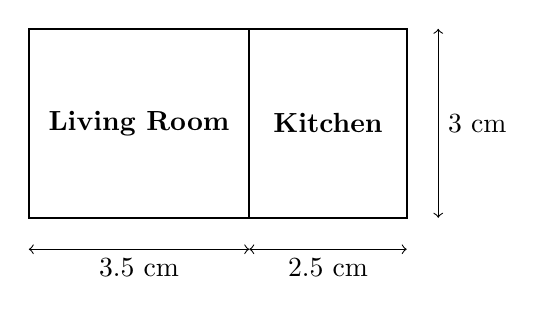
\begin{tikzpicture}[scale=0.8]
  \draw[thick] (0,0) rectangle (6,3);
  \draw[thick] (3.5,0) -- (3.5,3);
  \node at (1.75,1.5) {\textbf{Living Room}};
  \node at (4.75,1.5) {\textbf{Kitchen}};
  \draw[<->] (0,-0.5) -- (3.5,-0.5);
  \node[below] at (1.75,-0.5) {$3.5$ cm};
  \draw[<->] (3.5,-0.5) -- (6,-0.5);
  \node[below] at (4.75,-0.5) {$2.5$ cm};
  \draw[<->] (6.5,0) -- (6.5,3);
  \node[right] at (6.5,1.5) {$3$ cm};
\end{tikzpicture}
\end{center}
\end{questionText}
\choiceA{$3.5$ m}
\choiceB{$12.5$ m}
\choiceC{$15$ m}
\choiceD{$17.5$ m}
\correctAnswer{D}
\explanation{The living room is $3.5$ cm on the drawing. Actual length: $3.5 \times 5 = 17.5$ m.}
\end{practiceQuestion}

\begin{practiceQuestion}{6-1-q27}{gmc}
\begin{questionText}
The map below uses the scale $1$ cm $= 10$ km. What is the actual distance from Town A to Town C?

\begin{center}
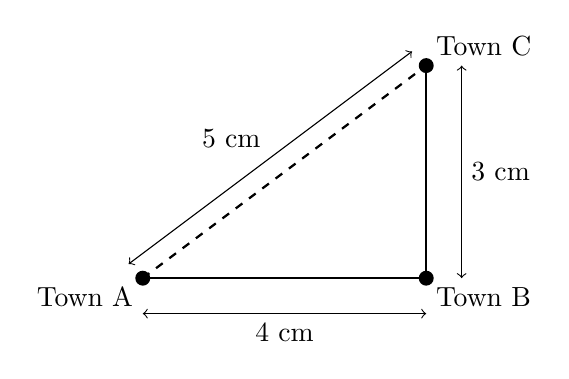
\begin{tikzpicture}[scale=0.9]
  \fill (0,0) circle (3pt) node[below left]{Town A};
  \fill (4,0) circle (3pt) node[below right]{Town B};
  \fill (4,3) circle (3pt) node[above right]{Town C};
  \draw[thick] (0,0) -- (4,0) -- (4,3);
  \draw[dashed,thick] (0,0) -- (4,3);
  \draw[<->] (0,-0.5) -- (4,-0.5);
  \node[below] at (2,-0.5) {$4$ cm};
  \draw[<->] (4.5,0) -- (4.5,3);
  \node[right] at (4.5,1.5) {$3$ cm};
  \draw[<->] (-0.2,0.2) -- (3.8,3.2);
  \node[above left] at (1.8,1.7) {$5$ cm};
\end{tikzpicture}
\end{center}
\end{questionText}
\choiceA{$30$ km}
\choiceB{$40$ km}
\choiceC{$50$ km}
\choiceD{$70$ km}
\correctAnswer{C}
\explanation{The direct distance from A to C on the map is $5$ cm. Actual distance: $5 \times 10 = 50$ km.}
\end{practiceQuestion}

\begin{practiceQuestion}{6-1-q28}{gmc}
\begin{questionText}
The scale drawing below shows a rectangular garden with scale $1$ cm $= 3$ m. Which statement is correct about the actual garden?

\begin{center}
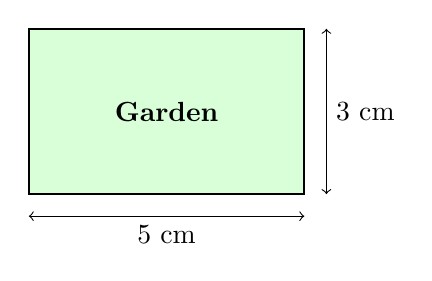
\begin{tikzpicture}[scale=0.7]
  \draw[thick,fill=green!15] (0,0) rectangle (5,3);
  \draw[<->] (0,-0.4) -- (5,-0.4);
  \node[below] at (2.5,-0.4) {$5$ cm};
  \draw[<->] (5.4,0) -- (5.4,3);
  \node[right] at (5.4,1.5) {$3$ cm};
  \node at (2.5,1.5) {\textbf{Garden}};
\end{tikzpicture}
\end{center}
\end{questionText}
\choiceA{The actual garden has an area of $15$ m$^2$}
\choiceB{The actual garden has a perimeter of $48$ m}
\choiceC{The actual garden has an area of $135$ m$^2$}
\choiceD{The actual garden has a perimeter of $16$ m}
\correctAnswer{C}
\explanation{Actual dimensions: $5 \times 3 = 15$ m and $3 \times 3 = 9$ m. Area: $15 \times 9 = 135$ m$^2$. Perimeter: $2(15 + 9) = 48$ m. Both B and C look plausible, but the area of $135$ m$^2$ matches choice C.}
\end{practiceQuestion}

\begin{practiceQuestion}{6-1-q29}{gsa}
\begin{questionText}
The scale drawing below shows an L-shaped room. The scale is $1$ cm $= 2$ m. What is the actual area of the room?

\begin{center}
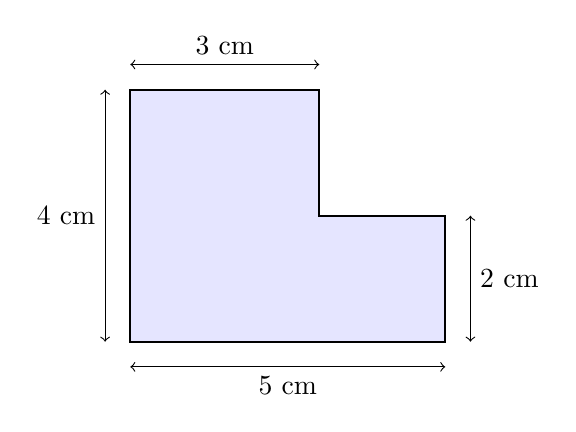
\begin{tikzpicture}[scale=0.8]
  \draw[thick,fill=blue!10] (0,0) -- (5,0) -- (5,2) -- (3,2) -- (3,4) -- (0,4) -- cycle;
  \draw[<->] (0,-0.4) -- (5,-0.4);
  \node[below] at (2.5,-0.4) {$5$ cm};
  \draw[<->] (5.4,0) -- (5.4,2);
  \node[right] at (5.4,1) {$2$ cm};
  \draw[<->] (-0.4,0) -- (-0.4,4);
  \node[left] at (-0.4,2) {$4$ cm};
  \draw[<->] (0,4.4) -- (3,4.4);
  \node[above] at (1.5,4.4) {$3$ cm};
\end{tikzpicture}
\end{center}
\end{questionText}
\correctAnswer{$64$ m$^2$}
\explanation{Split into two rectangles. Left: $3$ cm $\times$ $4$ cm $= 12$ cm$^2$. Bottom-right: $(5-3)$ cm $\times$ $2$ cm $= 4$ cm$^2$. Total drawing area: $16$ cm$^2$. Scale: $1$ cm $= 2$ m, so areas scale by $2^2 = 4$. Actual area: $16 \times 4 = 64$ m$^2$.}
\end{practiceQuestion}

\begin{practiceQuestion}{6-1-q30}{gsa}
\begin{questionText}
A scale drawing of a soccer field is shown on the grid below. Each grid square represents $10$ m $\times$ $10$ m in real life. What is the actual perimeter of the field?

\begin{center}
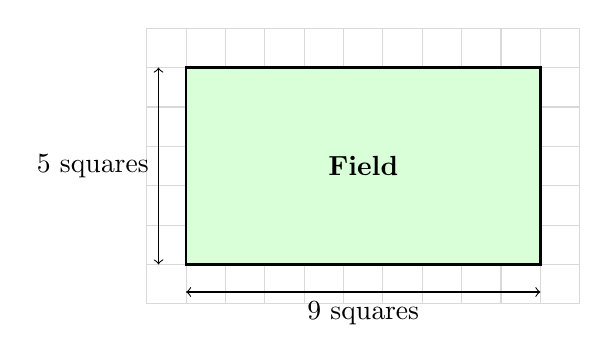
\begin{tikzpicture}[scale=0.5]
  \draw[step=1,gray!30,thin] (0,0) grid (11,7);
  \draw[thick,fill=green!15] (1,1) rectangle (10,6);
  \node at (5.5,3.5) {\textbf{Field}};
  \draw[<->] (1,0.3) -- (10,0.3);
  \node[below] at (5.5,0.3) {$9$ squares};
  \draw[<->] (0.3,1) -- (0.3,6);
  \node[left] at (0.3,3.5) {$5$ squares};
\end{tikzpicture}
\end{center}
\end{questionText}
\correctAnswer{$280$ m}
\explanation{Each square is $10$ m. Length: $9 \times 10 = 90$ m. Width: $5 \times 10 = 50$ m. Perimeter: $2(90 + 50) = 2(140) = 280$ m.}
\end{practiceQuestion}
